\chapter{Vergelijking Angular en Vaadin}
\label{ch:angular}
\section{Mobile}
In de afgelopen jaren is de ontwikkeling van mobiele applicaties een "booming business" geworden. Dankzij mobiele ondersteuning blijft een applicatie altijd en overal bereikbaar, het zorgt voor een direct marketingkanaal, een grotere merkherkenning, verhoogt het inkomen,... \\
 Alle voorgaande redenen en nog vele andere bepalen dat mobiele ondersteuning voor een framework belangrijk is.

\begin{figure}[H]
	\centering
	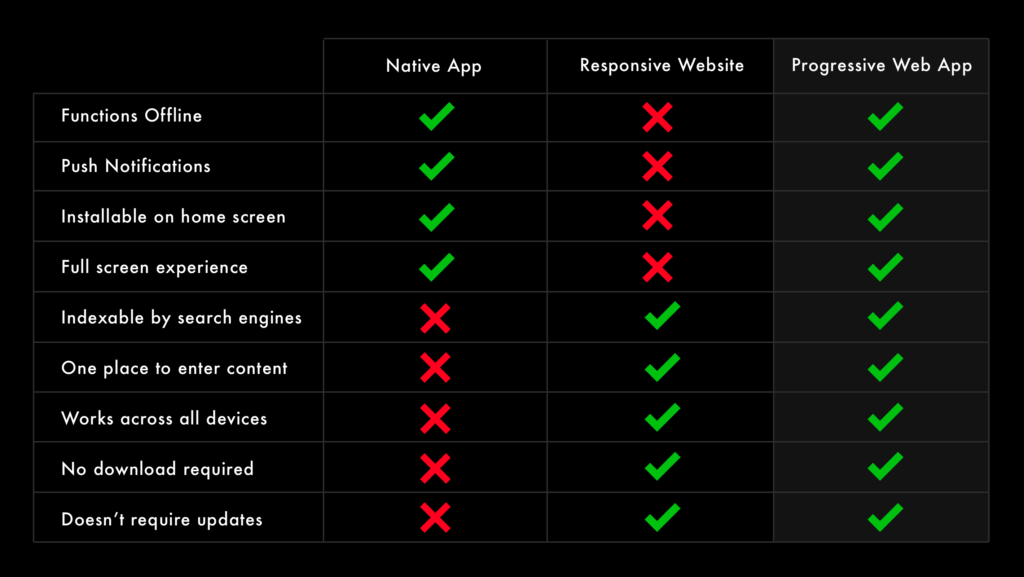
\includegraphics[width=0.6\linewidth]{Native-Web-progressive}
	\caption{Native App vs Responsive App vs Progressive App \autocite{Solis2018}}
	\label{fig:native-responsive-web}
\end{figure}
Bij het ontwikkelen van een mobiele applicatie heeft de ontwikkelaar drie opties(zie figuur \ref{fig:native-responsive-web}):
\begin{itemize}
	\item Responsive webapplicaties: De webapplicatie zal zich aanpassen aan het device waarop de applicatie wordt gedraaid. Deze aanpak is kostefficiënt omdat er maar een applicatie moet gebouwd worden voor zowel desktop als mobiele gebruikers. Verder is er geen download nodig, aangezien de webapplicaties gewoon via de browser kan opgeroepen worden.
	\item Native applicatie: De applicatie wordt specifiek gebouwd voor native platformen zoals iOS of Android. De voordelen van native applicaties is dat ze een betere performantie hebben, offline beschikbaar zijn en push notificaties kunnen sturen. Anderzijds moet elke applicatie gebouwd en getest worden voor elk ondersteund platform.
	\item Progressive webapplicaties(PWA):  Progressive webapplicaties zijn websites gebouwd met webtechnologie die zich gedragen als een app. Ze zijn de opvolgers van de hybride applicatie(een downloadbare app die de browser opstart en toont zonder navigatie) maar in tegenstelling tot de hybride applicatie vereisen ze geen download. Net als de native applicaties kunnen ze geraadpleegd worden zonder internetverbinding en kunnen ze push notificaties uitsturen. 
\end{itemize}

Vaadin en Angular hebben zeer verschillende aanpakken met betrekking tot mobiele ondersteuning. Waar de focus van Vaadin op het web ligt, zorgt Angular voor herbruikbaarheid van delen van de applicatie om mobiele applicaties te bouwen.
\subsection{Angular}
De ontwikkelaar heeft verschillende keuzes wanneer hij een mobiele applicatie wil ontwikkelen met Angular. Hij kan zowel een responsive webapplicatie als een progressive webapplicatie maken. Hij kan zelfs een native applicatie maken wanneer hij de template maakt met NativeScript in plaats van HTML. 

Het responsief maken van de applicatie gebeurt aan de hand van CSS media query's. Deze media query's staan de ontwikkelaar toe om verschillende regels voor de layout toe te voegen afhankelijk van de grootte van het scherm van het device. Verder kunnen de ontwikkelaars ook listeners toevoegen in de TypeScript code die reageren veranderingen in de grootte van het scherm. Zo kunnen bepaalde componenten veranderd worden als de grootte van het scherm verandert. 

\subsection{Vaadin}
Wanneer de ontwikkelaar ervoor kiest om de mobiele applicatie te bouwen in Vaadin heeft hij twee keuzes: een responsive webapplicatie of een progressive webapplicatie. 
Voor het ontwikkelen van een progressive webapplicatie zijn er vanuit technisch standpunt twee dingen noodzakelijk: een  Web App Manifest file en een ServiceWorker JavaScript file. De manifest file zorgt voor metadata zoals kleuren en iconen voor operating system integratie, de ServiceWorker zorgt voor caching en push notificaties.
Terwijl de ServiceWorker en de manifest file in Angular automatisch worden aangemaakt, moeten deze bij Vaadin manueel aangemaakt worden. Verder zal de applicatie ook niet offline beschikbaar zijn aangezien de application state wordt bijgehouden door de server.
Dit leidt ertoe dat het opzetten van een progressive webapplicatie in Vaadin moeilijker is en langer duurt.  
Vanaf de volgende versie van Vaadin (Vaadin 13) zou de ServiceWorker en de manifest file echter wel aan het framework toegevoegd worden. 
\subsection{Conclusie}
Angular zorgt voor een grotere flexibiliteit dan Vaadin bij het ontwikkelen van mobiele applicaties aangezien de developer ook kan opteren voor een native applicatie. Het ontwikkelen van een progressive webapplicatie verloopt bij Angular ook sneller en eenvoudiger dan bij Vaadin. Bovendien zal de Angular progressive webapplicatie ook offline beschikbaar zijn, waar dit voor een Vaadin progressive webapplicatie niet het geval is. Bovenstaande redenen zorgen ervoor dat Angular beter scoort dan Vaadin op het onderdeel mobile. \\
Angular krijgt voor deze requirement een score van 4, Vaadin een score van 2.

\section{Browsercompatibiliteit}
Browsercompatibiliteit is de manier waarop een webpagina er anders uitziet in verschillende webbrowsers. Verschillende browsers lezen de code van een website op een verschillende manier. Hierdoor zal Chrome een website soms anders weergeven dan FireFox of Internet Explorer. Voor een website is het belangrijk dat hij compatibel is met verschillende browsers omdat niet alle gebruikers dezelfde browser gebruiken. 
De browsercompatibiliteit van beide frameworks is weergegeven in tabel  \ref{table:browsercompatibiliteit}.

\subsection{Conclusie}
Beide frameworks zijn compatibel met alle populaire browsers. Daarom krijgen zowel Vaadin als Angular de maximumscore van 5 op deze requirement.


\begin{table}[H]
	\begin{tabular}{|l|l|l|l|l|l|}
		\hline
		\textbf{Framework} & \textbf{Chrome} & \textbf{FireFox} & \textbf{Internet Explorer} & \textbf{Edge}     & \textbf{Safari}   \\ \hline
		\textbf{Angular}   & Laatste versie  & Laatste versie   & 11,10,9                    & 2 laatste versies & 2 laatste versies \\ \hline
		\textbf{Vaadin}    & Laatste versie  & Laatste versie   & 11,10                      & Laatste versie    & Geen info         \\ \hline
	\end{tabular}
\caption{Compatibiliteit met browsers}
\label{table:browsercompatibiliteit}
\end{table}


\section{Data binding}
Het implementeren van data binding is belangrijk voor frameworks aangezien het heel wat tijd kan besparen. Er zijn verschillende soorten data binding die we voor elk framework zullen bespreken.
\\  \\
\textbf{one-way data binding} \hspace{1cm} Een aanpassing in het model zal automatisch de views/templates aanpassen.
\\ \\
\textbf{two-way data binding} \hspace{1cm} Het veranderen van de view resulteert in een verandering in het model en een verandering in het model resulteert in een aangepaste view. 
\\ \\
\textbf{three-way data binding} \hspace{1cm} De data wordt gesynchroniseerd met een  remote storage. 
\\ \\
\textbf{four-way data binding} \hspace{1cm} De data wordt gesynchroniseerd met een  lokale database, die op zijn beurt weer gesynchroniseerd wordt met een remote storage.

\subsection{Angular}

\subsubsection{one-way data binding}
\begin{figure}[H]
\begin{lstlisting}
<div>{{contact.voornaam}}</div>
\end{lstlisting}
\caption{One-way data binding Angular}
\end{figure}
\subsubsection{two-way data binding}

\begin{figure}[H]
\begin{lstlisting}
<input [(ngModel)]="contact.afbeelding"\>
\end{lstlisting}
\caption{Two-way data binding Angular}
\end{figure}
\subsubsection{three-way data binding}
Geen standaard implementatie, de ontwikkelaar moet dit zelf schrijven.

\subsubsection{four-way data binding}
Geen standaard implementatie, de ontwikkelaar moet dit zelf schrijven.
\subsection{Vaadin}
\subsubsection{one-way data binding}

\begin{figure}[H]
\begin{lstlisting}
<div>[[voornaam]]</div>
\end{lstlisting}
\caption{One-way data binding Vaadin}
\end{figure}
\subsubsection{two-way data binding}
\begin{figure}[H]
\begin{lstlisting}
<input value="{{voornaam::input}}">
\end{lstlisting}
\caption{Two-way data binding Vaadin}
\end{figure}

\subsubsection{three-way data binding}
Geen standaard implementatie, de ontwikkelaar moet dit zelf schrijven.
\subsubsection{four-way data binding}
Geen standaard implementatie, de ontwikkelaar moet dit zelf schrijven.

\subsubsection{Conclusie}
Beide frameworks hebben een eenvoudige implementatie van zowel one-way als two-way data binding. Beide frameworks kunnen zich nog verbeteren door het implementeren van three-way data binding en four-way data binding te vereenvoudigen. Hierdoor krijgen beide frameworks een score van 3. 

\section{Moeilijkheidsgraad}
Het aanleren van een framework is niet altijd eenvoudig. Hoe sneller een developer een framework onder de knie kan krijgen hoe beter. 
Angular is vrij moeilijk om aan te leren: de programmeur moet namelijk drie verschillende talen leren.
Eerst en vooral moet hij TypeScript leren. Hiervoor heeft hij een voorkennis nodig van JavaScript. Daarenboven moet hij ook een uitgebreide kennis hebben van HTML en CSS voor het maken en stylen van de templates.
\\
In tegenstelling tot Angular is Vaadin veel eenvoudiger om te leren. De programmeur moet enkel Java kennen, kennis van HTML en CSS is een pluspunt maar niet noodzakelijk.
Doordat er enkel kennis van Java nodig is, is Vaadin een framework dat gemakkelijk aangeleerd kan worden door programmeurs die geen ervaring hebben in de web-development sector.

\subsection{Conclusie}
Angular is een vrij moeilijk framework om aan te leren doordat de programmeur drie talen moet kennen. Vaadin is makkelijker onder de knie te krijgen aangezien applicaties geschreven kunnen worden met kennis van één taal, namelijk Java. 
Voor deze reden krijgt Vaadin een score van 4 en Angular een score van 2.


\section{Open source}
Open source software is software waarvan de broncode is gepubliceerd en vrij te gebruiken is voor het publiek. Iedereen kan op die manier kopiëren, aanpassen en verspreiden zonder kosten te betalen voor auteursrechten.
Bij de ontwikkeling van een webapplicatie of een mobiele applicatie is het dus voordelig wanneer de frameworks gratis gebruikt kunnen worden. 

\subsection{Angular} \label{Open source Angular}
Angular wordt aangeboden onder de MIT-licentie \autocite{MIT2019}.
De MIT-licentie is een softwarelicentie voor opensourcesoftware. Deze MIT-licentie staat bijna alles toe. De enige voorwaarde is dat het copyright statement in alle kopieën moet blijven staan.
De broncode van Angular is beschikbaar op: 
\\
\url{https://github.com/angular/angular} \\ \\
Verder zijn er ook heel veel voorgemaakte componenten waarvan de broncode beschikbaar is. Angular heeft zelf ook een library met componenten die ze beschikbaar stellen onder de naam Material Design. Net als het framework worden deze componenten aangeboden onder de MIT-licentie. De broncode van deze library kan gevonden worden op:
\\
\url{https://github.com/angular/components}

\subsection{Vaadin} \label{Open source Vaadin}
Vaadin Framework is beschikbaar onder de Apache License, version 2.0 \autocite{Apache2019}.
De Apache-licentie is een softwarelicentie voor vrije software uitgebracht door de Apache Software Foundation. De licentie staat toe dat deze software aangepast en/of opnieuw verspreid mag worden op voorwaarde dat een kopie van de Apache License wordt meegeleverd en de eerdere copyrightvermeldingen behouden blijven.
\\ De documentatie van het framework staat onder een andere licentie, namelijk de Creative Commons CC-BY-ND 2.0. Dit houdt in dat licentienemers  het werk mogen  kopiëren, verspreiden, tentoonstellen en uitvoeren en afgeleide werken maken wanneer zij de auteur of licentieverstrekker op een door deze gespecificeerde manier vermelden. Dit mag enkel gebeuren in ongewijzigde vorm.
\\De broncode van het framework kan gevonden worden op: 
\\ \url{https://github.com/vaadin/flow} \\ \\

Vaadin voorziet ook open source componenten onder de naam Vaadin core components. Deze worden net als het framework aangeboden onder de Apache License, version 2.0.
\\ De broncode van deze components is beschikbaar op 
\\ \url{https://github.com/vaadin/vaadin-core }

\subsection{Conclusie}
De MIT-licentie van Angular is kort en zeer eenvoudig. Alles mag aangepast worden aan de broncode op voorwaarde dat de originale licentie aanwezig blijft. 
De Apache License, version 2.0 waaronder Vaadin valt is net als de MIT-licentie een licentie dat heel veel toelaat. Het enige nadeel ten opzichte van de MIT-licentie is dat wanneer iets aangepast wordt aan de Apache-licensed code dit ook steeds moet aangegeven worden.
Aangezien dit maar een heel klein verschil betreft en beide frameworks in essentie volledig open source zijn, krijgen ze beiden de maximumscore van 5 op dit onderdeel.

\section{Testing}
Testen is een belangrijk onderdeel bij het bouwen van robuuste applicaties. Het zorgt ervoor dat fouten in de code op tijd worden opgevangen en geeft de ontwikkelaar vertrouwen in de werking van zijn applicatie. We zullen in dit onderdeel de focus leggen op UI tests aangezien andere tests niet framework specifiek zijn maar gebeuren aan de hand van gestandardiseerde tools zoals JUnit voor Java of Jasmine voor JavaScript.

\subsection{Angular}

\subsection{Vaadin}

\subsection{Conclusie}

\section{ Componenten}
Voorgemaakte componenten kunnen de ontwikkelaar heel veel tijd besparen. Ze zorgen bovendien ook voor een propere en consistente layout. Daarom wordt er in dit onderdeel ingegaan op het aantal beschikbare open source componenten. Deze componenten kunnen zowel aangeboden worden door de ontwikkelaars van het framework zelf als door een third party.

\subsection{Angular}
Zoals eerder vermeld in sectie \ref{Open source Angular} voorzien de ontwikkelaars van Angular hun gebruikers zelf met een library van voorgedefiniëerde componenten. Deze library heet Material Design en voorziet buttons, formulieren, menu's en nog veel meer. Deze UI components kunnen dienen als voorbeeld van hoe Angular code geschreven dient te worden volgens de best practices van het Angular team.
\\ \\
Daarenboven zijn er ook heel wat third party libraries beschikbaar. 
\begin{itemize}
	\item NGX Bootstrap: Bevat alle belangrijkste Bootstrap componenten.
	\item Prime NG: Meer dan 70 UI components die onder meer door eBay gebruikt worden. 
	\item Onsen UI: Focus op hybride en mobile web applicaties voor Android en iOS.
	\item NG-ZORRO: Chinese library geschreven in TypeScript.
	\item NG Lightning: Gebruikmakend van het Lightning Design System CSS framework.
	\item NG Semantic-UI: 27 Verschillende componenten.
	\item Clarity: ontwikkeld door VMware met een focus op data binding.
	\item NG2 Charts: 6 verschillende soorten charts voor het visualiseren van data en lists.
\end{itemize}

\subsection{Vaadin}
Bij het Vaadin framework voorzien de ontwikkelaars ook een library met componenten voor hun gebruikers onder de naam Vaadin core components. Dit werd eerder reeds vermeld in section \ref{Open source Vaadin}. Deze library bevat 78 verschillende componenten zoals buttons, date pickers, grids en vele anderen. 

Verder zijn er nog een paar, minder bekende third party libraries beschikbaar.
\begin{itemize}
	\item Material: Material stijl voor Vaadin 7 en 8.
	\item Vaadin Charts: Verschillende soorten charts die zorgen voor een betere visualisatie. 
\end{itemize}

\subsection{Conclusie}
De ontwikkelaars van beide frameworks voorzien hun gebruikers met een uitgebreide library van voorgedefiniëerde componenten. Het gebruik van deze componenten zorgt voor een responsief en consistent design. Angular beschikt hierboven nog over een groot aantal third party libraries. Dit is niet het geval bij Vaadin.
Daarom krijgt Vaadin een score van 3, terwijl Angular een score van 5 krijgt.

\section{Performantie}
De performantie van een framework is een belangrijke parameter bij een vergelijking omdat het inzicht verschaft in de werking van het framework. Het beantwoordt een aantal vragen zoals: hoe gaat het framework om met grote hoeveelheden data, hoe snel start het framework en wat is de belasting van de applicatie op de processor.

De tests worden allemaal uitgevoerd in dezelfde omgeving. De details van deze omgeving zijn als volgt:

\begin{itemize}
	
	\item Browser: Google Chrome Versie 74.0.3729.157 (Officiële build) (64-bits)
	\item Operating System: Microsoft Windows 10 Pro
	\item Fysiek geheugen: 16.0 GB RAM
	\item Processor: AMD FX(tm)-8350, 4000 MHz
\end{itemize}

De tests worden uitgevoerd op de applicaties die eerder beschreven zijn in sectie \ref{ch:methodologie}.

\subsection{Requests}
In dit onderdeel worden de groottes van de request die gedownload worden in de applicatie besproken. Om dit te controleren wordt er gebruik gemaakt van de Google Chrome Developer Tools Network Tab. De tests gebeurt bij het openen van de homepage van de applicatie.
\subsubsection{Angular}

\begin{table}[H]
	\begin{tabular}{|l|l|l|l|}
		\hline
		\textbf{Aantal requests} & \textbf{Grootte} & \textbf{Resources} & \textbf{Tijd om te laden} \\ \hline
		13                       & 2.5KB            & 5.3MB resources    & 967 ms                    \\ \hline
	\end{tabular}
\end{table}
\subsubsection{Vaadin}
\begin{table}[H]
	\begin{tabular}{|l|l|l|l|}
		\hline
		\textbf{Aantal requests} & \textbf{Grootte} & \textbf{Resources} & \textbf{Tijd om te laden} \\ \hline
		17                       & 12.9 KB          & 1.6MB resources    & 278 ms                    \\ \hline
	\end{tabular}
\end{table}

\subsection{Gebruik processor}

\subsubsection{Angular}
524.9 MB

\subsubsection{Vaadin}
322.7 MB

\section{Documentatie}
Het documenteren van frameworks is een belangrijk proces in de ontwikkeling van applicatie frameworks. Het is een voorwaarde die vervuld moet worden om een framework op een kwaliteitsvolle manier te kunnen gebruiken. Deze documentatie moet niet enkel uitgebreid zijn, maar ook makkelijk begrijpbaar, accuraat en up-to-date zijn. Goede documentatie is bovendien dynamisch: het maakt gebruik van geavanceerde visualisatie technieken zoals voorbeeldcode, afbeeldingen en video's. Dit in tegenstelling tot de verouderde statische documentatie zoals die de opbouw van een kookboek volgen. 

\subsection{Angular}
De documentatie van Angular \autocite{Angular2019} is zeer uitgebreid (16.5 MB) en is eenvoudig vindbaar op de website van Angular of via een zoekmachine. De documentatie volgt de chronologische opbouw van een applicatie. Zo start de documenatie met een "Getting started" pagina waar getoond wordt welke installaties moeten gebeuren en hoe het genereren van een project gebeurt. 
Hierna volgt een tutorial waarin een voorbeeldapplicatie rond superhelden wordt opgebouwd in zes stappen. \\ Na de tutorial volgt een onderdeel waarin de "Fundamentals" van het Angular framework worden uitgelegd. Hierin geeft de documentatie ondermeer informatie over het implementeren van formulieren en navigatie. \\
Vervolgens worden een aantal belangrijke technieken overlopen zoals service workers en security.  \\
Na de technieken gaat men over naar setup en deployment. Hier behandelt de documentatie onderdelen zoals testing, TypeScript configuratie en npm dependencies. Na dit onderdeel heeft de gebruiker in principe alle informatie die hij nodig heeft om een volledige applicatie op te bouwen.\\
Ten slotte volgen nog enkele algemene onderdelen met informatie rond releases, referenties en CLI commands. 

De documentatie zit vol met afbeeldingen en code snippets, maar er zijn geen video's of audiofragmenten aanwezig. Indien de gebruiker hiervan gebruik wil maken moet hij gebruik maken van third-party documentatie zoals video's op video sharing websites of podcasts. De documentatie is bovendien enkel online beschikbaar, deze downloaden in PDF formaat is niet mogelijk. 

\subsection{Vaadin}
Documenatie bij Vaadin is uitgebreid(1.5 MB) en eenvoudig vindbaar op de website van Vaadin of via een zoekmachine. De flow van deze documenatie is chronologisch opgedeeld, waarbij er gestart wordt met een overzicht en een introductie. \\
Na deze introductie worden verschillende stappen gevolgd om een applicatie op te bouwen. Het eerste onderdeel handelt rond navigatie. Hierna volgen enkele algemene onderdelen zoals browser features, het gebruik van components en data binding. \\ 
Tot hiertoe heeft de documentatie het enkel over Java. In de volgende stap wordt er uitgelegd hoe je HTML, JavaScript en CSS files kan koppelen aan de applicatie. 
Hierna volgen enkele onderdelen in verband met de opmaak van de applicatie zoals het thematiseren van de applicatie voor een consistente layout, het creëren van componenten, het integreren van web componenten en het creëren van templates. \\
Hierna volgen nog enkele algemene onderdelen zoals onder andere: integreren van Spring of CDI, packaging voor productie of het migreren van Vaadin 8 naar Vaadin 10. \\

Er zijn volop code snippets en afbeeldingen aanwezig, maar ook hier zijn er geen video's of audiofragmenten. Deze zijn wel beschikbaar via een third-party op andere kanalen, maar de correctheid van deze bronnen is niet altijd te controleren. De documenatie is enkel online beschikbaar.

\subsection{Conclusie}
Hoewel de documentatie van Angular een pak groter is dan die van Vaadin kan er niet geconcludeerd worden dat deze beter is. Beide frameworks beschikken over een uitgebreide documentatie die goed gevisualiseerd wordt met code snippets en afbeeldingen. Het enige opmerkbare verschil is dat Angular werkt met een tutorial applicatie in hun documentatie. Vaadin stelt ook een voorbeeld applicatie ter beschikking op hun Github \autocite{VaadinDemo2019}, maar deze is niet verwerkt in hun documentatie.

Beide frameworks verwerken geen video's of audiofragmenten in hun documentatie, die bovendien niet offline beschikbaar is. Hierdoor krijgen beide frameworks een score van 3.


\section{Aantal programmeertalen}



\section{Populariteit}
De populariteit is een belangrijk criterium bij het beoordelen van een framework. Een framework met veel gebruikers heeft een grote community, waardoor het vinden van oplossingen bij problemen makkelijker verloopt dan bij een framework met een kleine community. Daarenboven bepaalt het aantal gebruikers ook de stabiliteit van een framework. Ten slotte bepaalt de populariteit ook het aantal library's die door de community ter beschikking gesteld worden.
\subsection{Stack Overflow}
Stack Overflow is een platform dat als doel heeft om programmeurs te voorzien van een goede Q\&A website. Maandelijks heeft Stack Overflow meer dan 50 miljoen bezoekers waardoor het de grootste online developer community genoemd mag worden. 
\subsubsection{Angular}
Zie tabel \ref{table:angularstackoverflow}(raadpleging op 8/04/2019) op pagina \pageref{table:angularstackoverflow}. \\ \\
Angular heeft een heel groot aantal aangemaakte issues wat erop wijst dat Angular een zeer populair framework is. Het percentage opgeloste issues ligt rond de 60 percent, wat een redelijk goede score is.
\begin{table}[H]
	\begin{tabular}{|l|l|l|l|}
		\hline
		Naam van de tag   & \textbf{Aantal aangemaakte issues} & \textbf{Aantal onopgeloste issues} & \textbf{\% opgeloste issues} \\ \hline
		\textbf{Angular}  & 161.326                            & 65.823                             & 59,20\%                              \\ \hline
		\textbf{Angular5} & 2.827                              & 1.193                              & 57,80\%                              \\ \hline
		\textbf{Angular6} & 2.763                              & 1.181                              & 57,26\%                              \\ \hline
		\textbf{Angular7} & 723                                & 320                                & 55,74\%                              \\ \hline
		\textbf{Totaal}   & \textbf{167.639}                   & \textbf{68.517}                    & \textbf{59.13\%}                     \\ \hline
	\end{tabular}
\caption{Populariteit van Angular op Stack Overflow}
\label{table:angularstackoverflow}
\end{table}
\subsubsection{Vaadin}
Zie tabel \ref{table:vaadinstackoverflow}(raadpleging op 8/04/2019) op pagina \pageref{table:vaadinstackoverflow}. \\ \\
Het aantal aangemaakte issues van Vaadin ligt laag. Dit wijst erop dat Vaadin niet veel gebruikers heeft. Het percentage opgeloste issues ligt echter zeer hoog, namelijk rond de 84 percent. Ondanks de kleinere omvang van community is de kans op een oplossing van een issue dus toch groot. \\

\begin{table}[H]
	\begin{tabular}{|l|l|l|l|}
		\hline
		Naam van de tag   & \textbf{Aantal aangemaakte issues} & \textbf{Aantal onopgeloste issues} & \textbf{\% opgeloste issues} \\ \hline
		\textbf{Vaadin}  & 4.588                            & 691                             & 84,94\%                              \\ \hline
		\textbf{Vaadin6} & 9                              & 1                              & 88,89\%                              \\ \hline
		\textbf{Vaadin7} & 386                              & 85                              & 77,98\%                              \\ \hline
		\textbf{Vaadin8} & 166                                & 49                                & 70,48\%                              \\ \hline
		\textbf{Vaadin10} & 36                                & 12                                & 66,66\%                              \\ \hline
		\textbf{Totaal}   & \textbf{5.185}                   & \textbf{838}                    & \textbf{83.84\%}                     \\ \hline
	\end{tabular}
	\caption{Populariteit van Vaadin op Stack Overflow}
	\label{table:vaadinstackoverflow}
\end{table}

\subsection{Reddit}
Reddit is een social sharing website waarbij gebruikers zelf de content aanleveren. Dit kunnen zowel artikels als afbeeldingen of video's zijn. Reddit bestaat uit verschillende subreddits die handelen over bepaalde onderwerpen. Het aantal subscribers van deze subreddits kunnen een indicator vormen voor de populariteit van het onderwerp.\\

Uit de gegevens van tabel \ref{table:reddit} kunnen we afleiden dat Angular veel populairder is dan Vaadin. Met meer dan 200 keer meer subscribers is het verschil zeer duidelijk. Bovendien is de subreddit r/vaadin ook veel minder actief dan r/angular.
\begin{table}[H]
	\begin{tabular}{|l|l|l|}
		\hline
		\textbf{Subreddit}  & \textbf{Aantal subscribers} & \textbf{Aantal posts in de laatste 30 dagen} \\ \hline
		\textbf{r/angular2} & 31.468                      & 79                                           \\ \hline
		\textbf{r/vaadin}   & 147                         & 0                                            \\ \hline
	\end{tabular}
	\caption{Populariteit van de frameworks op Reddit}
\label{table:reddit}
\end{table}

\subsection{Stack Overflow Developer Survey}
Elk jaar voert Stack Overflow zijn Developer Survey \autocite{DeveloperSurvey2019} uit, waarbij duizenden developers vertellen over wat ze leren, welke tools en frameworks ze gebruiken en welke job ze uitvoeren. De resultaten hiervan kunnen gebruikt worden om de populariteit te bepalen van deze onderdelen. Door de resultaten de afgelopen jaren te gebruiken kan men bovendien een inzicht krijgen in de evolutie van de populariteit.


\subsubsection{Resultaten 2017}
In 2017 was Angular het tweede meest gebruikte framework, met maar liefst 44 percent van de respondenten die reeds het framework gebruikt hadden. Bovendien vonden meer dan de helft van de gebruikers het een leuk framework om te gebruiken.

Vaadin werd niet genoemd in deze enquête wat erop wijst dat het in 2017 geen populair.

\begin{figure}[H]
	\centering
	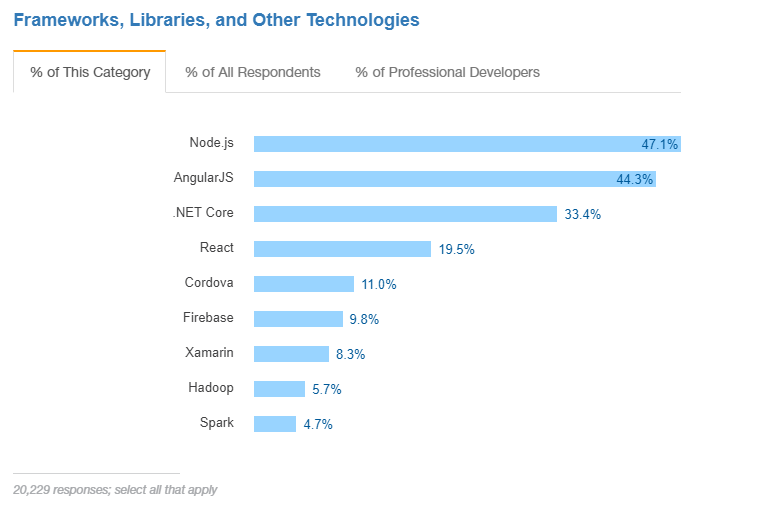
\includegraphics[width=0.6\linewidth]{2017Frameworks}
	\caption{Frameworks, Libraries, and Other Technologies 2017 \autocite{DeveloperSurvey2017}}
	\label{fig:Frameworks, Libraries, and Other Technologies 2017}
\end{figure}

\begin{figure}[H]
	\centering
	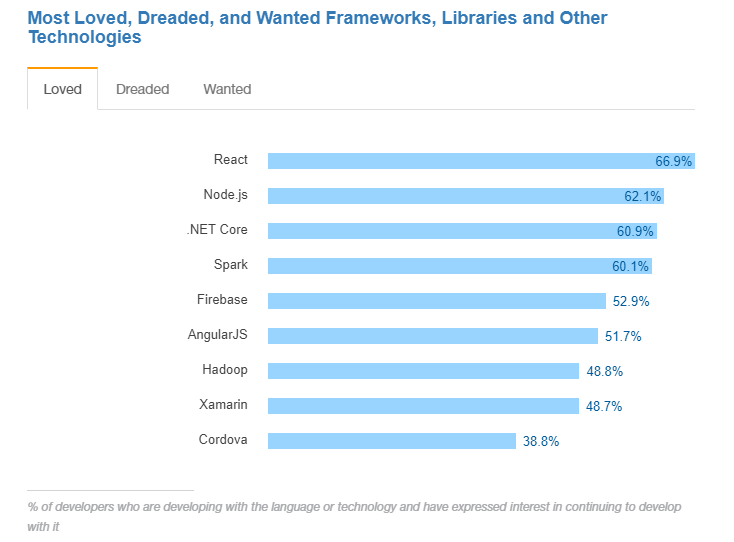
\includegraphics[width=0.6\linewidth]{2017LovedFrameworks}
	\caption{Most Loved Frameworks, Libraries and Other Technologies 2017 \autocite{DeveloperSurvey2017}}
	\label{fig:Most Loved Frameworks, Libraries and Other Technologies 2017}
\end{figure}

\subsubsection{Resultaten 2018}
In 2018 was Angular nog steeds het tweede meest gebruikte framework, maar het aantal respondenten die er al gebruik van gemaakt hadden daalde naar 37 percent. Nog steeds vonden meer dan de helft van de gebruikers het een leuk framework om te gebruiken.

Vaadin werd niet genoemd in deze enquête wat erop wijst dat het in 2018 geen populair framework was.

\begin{figure}[H]
	\centering
	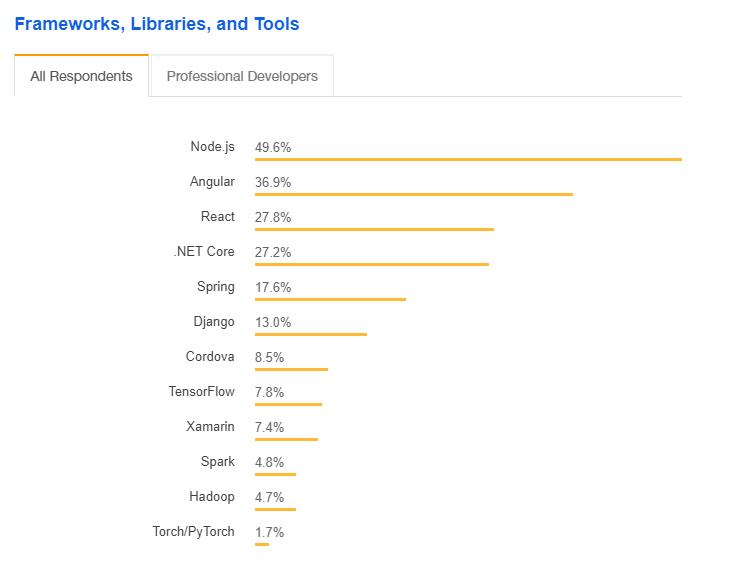
\includegraphics[width=0.6\linewidth]{2018Frameworks}
	\caption{Frameworks, Libraries, and Other Technologies 2018 \autocite{DeveloperSurvey2018}}
	\label{fig:Frameworks, Libraries, and Other Technologies 2018}
\end{figure}

\begin{figure}[H]
	\centering
	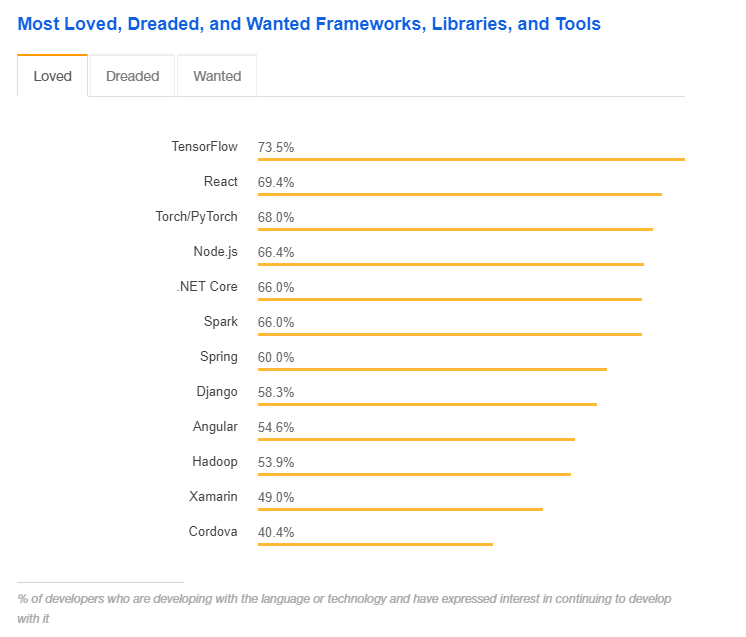
\includegraphics[width=0.6\linewidth]{2018LovedFrameworks}
	\caption{Most Loved Frameworks, Libraries and Other Technologies 2018 \autocite{DeveloperSurvey2018}}
	\label{fig:Most Loved Frameworks, Libraries and Other Technologies 2018}
\end{figure}

\subsubsection{Resultaten 2019}
De daling van de populariteit van Angular zette zich ook in 2019 verder. Het zakte van de tweede naar de derde plaats van populairste framework. Het aantal respondenten die gebruik maakten van het framework zakte naar 31 percent. Nochtans steeg het percentage van ontwikkelaars die er graag gebruik van maken naar 57 percent.

Vaadin werd niet genoemd in deze enquête wat erop wijst dat het in 2019 geen populair framework is.

\begin{figure}[H]
	\centering
	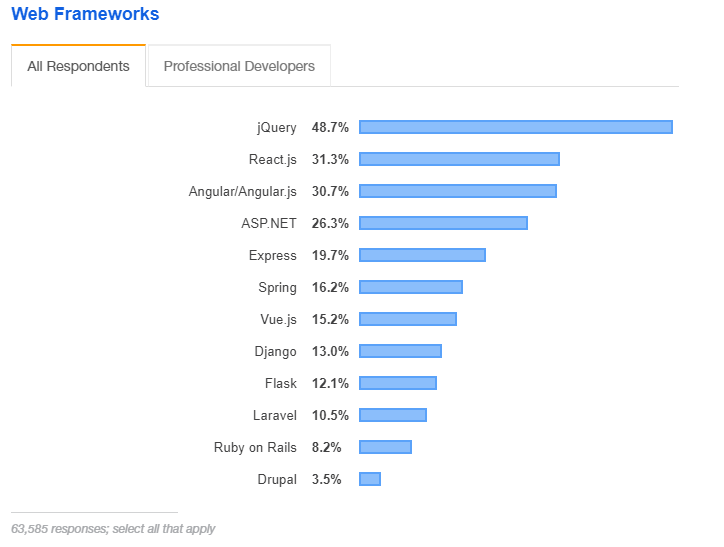
\includegraphics[width=0.6\linewidth]{2019Frameworks}
	\caption{Frameworks, Libraries, and Other Technologies 2019 \autocite{DeveloperSurvey2019}}
	\label{fig:Frameworks, Libraries, and Other Technologies 2019}
\end{figure}

\begin{figure}[H]
	\centering
	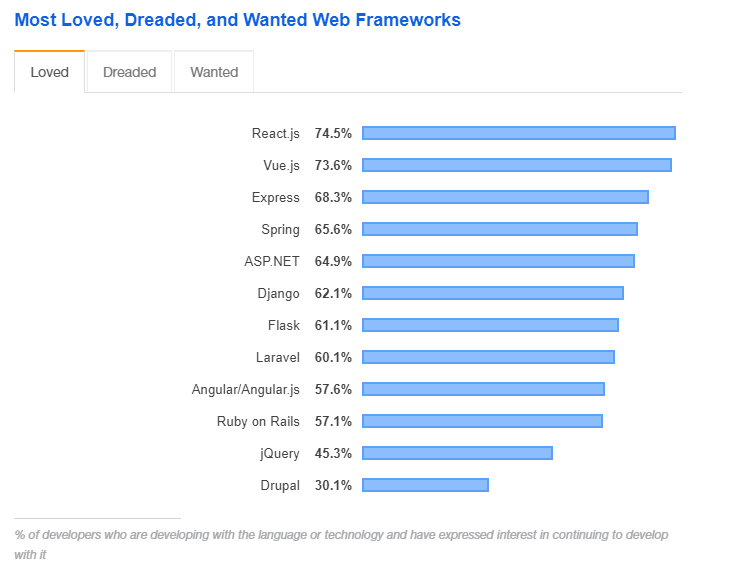
\includegraphics[width=0.6\linewidth]{2019LovedFrameworks}
	\caption{Most Loved Frameworks, Libraries and Other Technologies 2019 \autocite{DeveloperSurvey2019}}
	\label{fig:Most Loved Frameworks, Libraries and Other Technologies 2019}
\end{figure}

\subsection{Google Trends}

Google Trends is een dienst van Google die via grafieken inzicht geeft wanneer en hoe vaak op een bepaald woord is gezocht met Google. \\ \\
De cijfers in figuur \ref{fig:Google Trends zoektermen} geven de zoekinteresse aan ten opzichte van het hoogste punt in het diagram voor de betreffende regio en periode. Een waarde van 100 is de piekpopulariteit voor die term. Een waarde van 50 betekent dat de term half zo populair is. Een score van 0 betekent dat er onvoldoende gegevens beschikbaar zijn voor deze term. De resultaten van de zoekterm "Angular" worden weergegeven door een rode lijn, de resultaten van de zoekterm "Vaadin" door een blauwe lijn.

Er kan geconcludeerd worden dat er wereldwijd veel vaker gezocht wordt naar het sleutelwoord "Angular" dan naar "Vaadin". 

\begin{figure}[H]
	\centering
	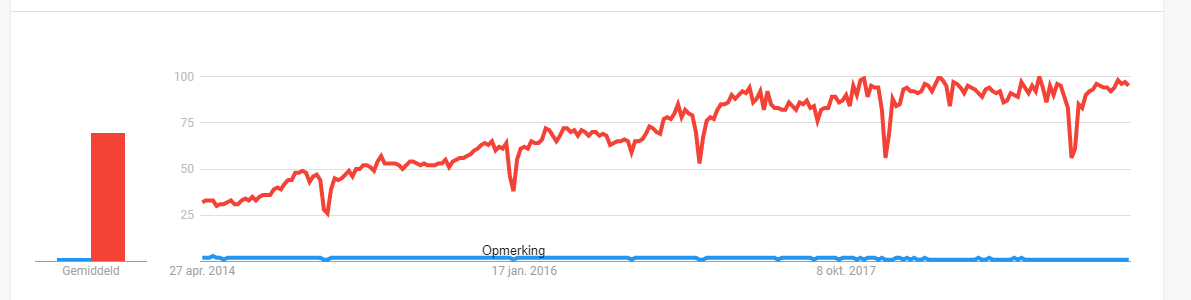
\includegraphics[width=0.6\linewidth]{GoogleTrendsTimeLine}
	\caption{Zoektermen Vaadin versus Angular \autocite{GoogleTrends2019}}
	\label{fig:Google Trends zoektermen}
\end{figure}

\subsection{Github}
GitHub is een populaire website waarop software kan geplaatst worden. GitHub is gebouwd rond het Git-versiebeheersysteem, waardoor GitHub alle mogelijkheden van Git en eigen toevoegingen aanbiedt. Het aantal watchers, stars en forks van een framework op Github is een indicator voor de populariteit van het framework. In tabel \ref{table:github} wordt nogmaals duidelijk dat Angular veel populairder is dan Vaadin.

\begin{table}[H]
	\begin{tabular}{|l|l|l|l|}
		\hline
		\textbf{Github}  & \textbf{Aantal watchers} & \textbf{Aantal stars} & \textbf{Aantal forks} \\ \hline
		\textbf{Angular} & 3284                     & 47.296                & 12.612                \\ \hline
		\textbf{Vaadin}  & 57                       & 184                   & 55                    \\ \hline
	\end{tabular}
	\caption{Populariteit van de frameworks op Github}
\label{table:github}
\end{table}

\subsection{Conclusie}
Angular is duidelijk veel populairder dan Vaadin, waardoor het framework stabieler is en de gebruiker kan rekenen op meer ondersteuning vanuit de community. Angular behoort tot de meest populaire frameworks, terwijl Vaadin niet populair is. De enige factor waar Vaadin beter op scoort dan Angular is het percentage opgeloste issues op Stack Overflow. 

Door de hierboven genoemde redenen krijgt Angular voor dit requirement een score van 5 en Vaadin een score van 2.



 